\documentclass[11pt,a4paper]{article}

\usepackage[utf8]{inputenc}
\usepackage[T1]{fontenc}
\usepackage{mathpazo}
\usepackage[scaled=0.95]{helvet}
\renewcommand{\ttdefault}{pcr}
\usepackage[a4paper,margin=25mm]{geometry}
\usepackage{microtype}
\usepackage{amsmath,amssymb}
\usepackage{booktabs}
\usepackage{array}
\usepackage[section]{placeins}
\usepackage{graphicx}
\usepackage{caption}
\usepackage{subcaption}
\usepackage{xcolor}
\usepackage{enumitem}
\usepackage{tikz}
\usetikzlibrary{arrows.meta,positioning,calc}
\usepackage{titlesec}
\usepackage{fancyhdr}
\usepackage[hidelinks]{hyperref}

% Generated by make report from results/results.json. Do not edit.
\newcommand{\valCorpus}{libri}
\newcommand{\valNUtt}{24}
\newcommand{\valNOwn}{6}
\newcommand{\valNCases}{1320}
\newcommand{\valNNoise}{11}
\newcommand{\valNSnr}{5}
\newcommand{\valSnrGrid}{$-$5, 0, 5, 10, 15}
\newcommand{\valNTune}{220}
\newcommand{\valActive}{83}
\newcommand{\valTestEvals}{1}
\newcommand{\valDsnrBone}{5.20}
\newcommand{\valDsnrBtwo}{0.52}
\newcommand{\valDsnrBthree}{$-$1.93}
\newcommand{\valDsnrBfour}{4.74}
\newcommand{\valDsnrBfive}{5.44}
\newcommand{\valDsnrBfiveLo}{4.81}
\newcommand{\valDsnrBfiveHi}{6.01}
\newcommand{\valSegBone}{3.03}
\newcommand{\valSegBfive}{3.54}
\newcommand{\valNrBone}{9.5}
\newcommand{\valNrBthree}{21.3}
\newcommand{\valNrBfive}{10.0}
\newcommand{\valMnrBone}{2.16}
\newcommand{\valMnrBfour}{1.98}
\newcommand{\valMnrBfive}{2.56}
\newcommand{\valPesqBone}{0.24}
\newcommand{\valPesqBthree}{$-$0.21}
\newcommand{\valPesqBfive}{0.25}
\newcommand{\valPesqBfiveCi}{0.25 [0.23, 0.27]}
\newcommand{\valStoiBthree}{$-$0.035}
\newcommand{\valStoiBfive}{0.003}
\newcommand{\valDsnrFiveAtLow}{7.4}
\newcommand{\valDsnrFiveAtHigh}{2.9}
\newcommand{\valSnrLow}{$-$5}
\newcommand{\valSnrHigh}{15}
\newcommand{\valMedDsnrOne}{0.26}
\newcommand{\valMedSegOne}{0.55}
\newcommand{\valMedDsnrFour}{0.75}
\newcommand{\valMedPesqFour}{0.08}
\newcommand{\valPPesqOne}{0.415}
\newcommand{\valPDsnrOne}{$<$0.001}
\newcommand{\valTransientFive}{$-$0.2}
\newcommand{\valBabbleOne}{1.4}
\newcommand{\valBabbleFive}{1.1}
\newcommand{\valBiquadLoss}{4.4}
\newcommand{\valNoneLoss}{1.7}
\newcommand{\valRiseOffDsnr}{5.55}
\newcommand{\valRiseOffNr}{16.6}
\newcommand{\valRiseOffSeg}{0.3}
\newcommand{\valPRiseOff}{0.604}
\newcommand{\valMinstatsGain}{0.1}
\newcommand{\valPMinstats}{0.011}
\newcommand{\valFanNrFive}{2.8}
\newcommand{\valFanNrOne}{3.9}
\newcommand{\valCorNrFive}{1.9}
\newcommand{\valCorNrOne}{2.1}
\newcommand{\valFanMixNr}{9.0}
\newcommand{\valCorMixNr}{9.2}
\newcommand{\valFanLevelThree}{$-$9.8}
\newcommand{\valCorLevelThree}{$-$11.3}
\newcommand{\valOwnDsnrFive}{5.53 [4.34, 6.31]}
\newcommand{\valOwnDsnrOne}{5.12}
\newcommand{\valJDevFive}{5.06}
\newcommand{\valJDevOne}{4.65}
\newcommand{\valJTestFive}{4.49}
\newcommand{\valJTestOne}{4.11}
\newcommand{\valGMin}{0.03}
\newcommand{\valGainMu}{0}
\newcommand{\valDdAlpha}{0.9}
\newcommand{\valMcraDelta}{3}
\newcommand{\valRiseLimit}{3}
\newcommand{\valOneA}{1}
\newcommand{\valOneGMin}{0.05}
\newcommand{\valDelayMs}{31.9}
\newcommand{\valDelaySamples}{511}
\newcommand{\valBlockBudget}{16}
\newcommand{\valRtf}{0.020}
\newcommand{\valWorstBlock}{0.56}
\newcommand{\valHeapKb}{102}
\newcommand{\valStreamDiff}{0}
\newcommand{\valAliasNaive}{0.0}
\newcommand{\valAliasFiltered}{$-$68.1}
\newcommand{\valAliasHz}{5000}
\newcommand{\valSqnrSixteen}{98.1}
\newcommand{\valSqnrSixteenQuiet}{58.1}
\newcommand{\valSqnrEightQuiet}{9.9}
\newcommand{\valCommit}{591a908}
\newcommand{\valGenerated}{2026-11-04}
\newcommand{\valPythonVersion}{3.11.18}
\newcommand{\valNumpyVersion}{2.4.6}
\newcommand{\valScipyVersion}{1.17.1}
\newcommand{\valPesqVersion}{0.0.4}
\newcommand{\valStoiVersion}{0.4.1}
\newcommand{\valNoisereduceVersion}{3.0.3}
\newcommand{\valTuningHash}{5faa0613f52ab9d5}

\graphicspath{{../results/figures/}}

\definecolor{ink}{HTML}{1d3fbb}
\setlist{itemsep=2pt,topsep=4pt}
\setlength{\parindent}{0pt}
\setlength{\parskip}{6pt}
\captionsetup{font=small,labelfont=bf,labelsep=period}
\titleformat{\section}{\sffamily\Large\bfseries}{\thesection}{0.8em}{}
\titleformat{\subsection}{\sffamily\large\bfseries}{\thesubsection}{0.8em}{}
\titleformat{\subsubsection}{\sffamily\normalsize\bfseries}{\thesubsubsection}{0.8em}{}
\pagestyle{fancy}
\fancyhf{}
\fancyhead[L]{\sffamily\small HushWave}
\fancyhead[R]{\sffamily\small Single-channel speech noise reduction}
\fancyfoot[C]{\sffamily\small\thepage}
\renewcommand{\headrulewidth}{0.3pt}
\renewcommand{\arraystretch}{1.12}

\newcommand{\dB}{\,dB}
\newcommand{\file}[1]{\texttt{#1}}
\DeclareMathOperator*{\argmin}{arg\,min}

\begin{document}

% ------------------------------------------------------------------ title
\begin{titlepage}
\sffamily
\vspace*{18mm}
{\color{ink}\rule{40mm}{1.2pt}}\par
\vspace{6mm}
{\fontsize{34}{38}\selectfont\bfseries HushWave\par}
\vspace{4mm}
{\Large Single-channel speech noise reduction\\[2pt] built from first principles in the STFT domain\par}
\vspace{16mm}
{\large DSP mini project 6\par}
\vspace{2mm}
Third-year B.Tech, Electronics and Communication Engineering\\
National Institute of Technology Goa
\vspace{14mm}

{\large\bfseries Group}\par\vspace{2mm}
\begin{tabular}{@{}ll@{}}
Roll No. 20 & Kartikey Tiwari \\
Roll No. 21 & \\
Roll No. 22 & \\
\end{tabular}

\vfill
\small
Repository: \file{github.com/kartikeyy12/hushwave-speech-denoiser}\\
Code revision \valCommit, results generated on \valGenerated\\
Every number in this report is produced by code and read from \file{results/results.json}.
\end{titlepage}

\begin{abstract}
\noindent
HushWave reduces stationary and slowly varying background noise in single-channel speech.
The signal path is a 16~kHz, 32~ms short-time Fourier transform with weighted overlap-add,
a noise power tracker (minima-controlled recursive averaging with a rise-rate limit), a
decision-directed Wiener gain, and a zero-phase spectral high-pass. The radix-2 FFT, the
windows, the STFT and overlap-add, the biquad, the trackers, the gain rules, the metrics, and
the Welch estimator are all implemented in the project; libraries are used only for file
input and output, plotting, special functions, and clearly marked external references.

The system was tuned on a development set and evaluated once on a held-out test set of
\valNUtt{} LibriSpeech utterances mixed with \valNNoise{} noise conditions at \valNSnr{} input
SNRs (\valNCases{} cases). Its mean SNR improvement is \valDsnrBfive\dB{} (95\% interval
\valDsnrBfiveLo{} to \valDsnrBfiveHi\dB), against \valDsnrBone\dB{} for tuned spectral
subtraction, \valDsnrBfour\dB{} for a Wiener gain without decision-directed estimation,
\valDsnrBtwo\dB{} for \file{scipy.signal.wiener}, and \valDsnrBthree\dB{} for a general-purpose
library denoiser. The margin over spectral subtraction is small but consistent
(median \valMedDsnrOne\dB, Holm-corrected $p$~\valPDsnrOne). Perceptual quality (PESQ-WB) is
equal to spectral subtraction, and no gain-based method improves STOI.
On two real recordings without a clean reference the noise reduction in pauses is only
\valFanNrFive\dB{} and \valCorNrFive\dB, no better than spectral subtraction. The streaming
engine has a fixed algorithmic delay of \valDelayMs~ms and runs at \valRtf{} of real time on the
measurement machine. A browser-based demonstration offers a replay mode and a live microphone mode.
\end{abstract}

\tableofcontents
\clearpage

% ------------------------------------------------------------------ 1
\section{Introduction}

\subsection{Problem and scope}
A microphone picks up speech together with fans, traffic, ventilation, and other people. When
only one microphone is available there is no spatial information to exploit, so the separation
has to rely on the statistics of the two signals: speech is non-stationary, sparse in time and
frequency, and harmonic; many environmental noises are close to stationary over a second or
more. The classical answer is short-time spectral attenuation. The signal is cut into
overlapping frames, a noise power spectrum is tracked, and each time-frequency cell is
multiplied by a gain that depends on how far its power rises above the noise.

The project brief, set by the course instructors, asks for an implementation of at least one DSP
algorithm by the students themselves (not only library calls), the mathematical formulation,
time-domain and frequency-domain analysis, raw against processed signals with numerical
measures, a justified sampling frequency, and a working real-time or near-real-time
demonstration. Appendix~\ref{app:trace} maps each requirement to the place in this report and
in the repository where it is met.

\subsection{What was built}
\begin{itemize}
\item A complete enhancement engine in \file{src/hushwave/}: radix-2 FFT, windows, STFT with
weighted overlap-add, biquad filter, two noise trackers, four gain rules, and the evaluation
metrics, each implemented from its definition.
\item A streaming implementation with a fixed delay, shown to produce the same samples as the
batch implementation (largest difference \valStreamDiff).
\item A reproducible experiment with separate development and test data, utterance-level
confidence intervals, and corrected significance tests.
\item A demonstration interface with a replay mode and a live microphone mode.
\end{itemize}

\subsection{Rules the project follows}
Three rules shape everything below.
\begin{enumerate}
\item \textbf{From scratch.} All algorithms of the signal path and the metrics are implemented
in the project. External code is limited to reading and writing files, plotting, special
functions, and the reference implementations used for comparison and for two perceptual metrics
(\file{pesq}, \file{pystoi}, \file{noisereduce}, \file{scipy.signal.wiener}). No learned model is used.
\item \textbf{No typed numbers.} Every number in this report, and every table, is generated by
code from \file{results/results.json}. Before a report is built, a script checks the
qualitative statements of the text against the data and stops if one no longer holds.
\item \textbf{One test evaluation.} Parameters were chosen on development data only. The test set
was evaluated once (\valTestEvals{} recorded evaluation, tuning file hash prefix \valTuningHash).
A second evaluation is refused by the code unless forced, and would have to be disclosed.
\end{enumerate}

% ------------------------------------------------------------------ 2
\section{Signal model and sampling}
\label{sec:model}

\subsection{Model}
The microphone signal is modelled as the sum of speech $s[n]$ and additive noise $d[n]$:
\begin{equation}
y[n] = s[n] + d[n].
\end{equation}
Speech and noise are assumed uncorrelated. The enhancement goal is an estimate $\hat s[n]$ with
less noise and as little change to the speech as possible. The input signal-to-noise ratio of a
mixture is
\begin{equation}
\mathrm{SNR}_\mathrm{in} = 10\log_{10}\frac{\sum_n s^2[n]}{\sum_n d^2[n]}.
\end{equation}
Test mixtures are built by scaling the noise by $g=\sqrt{\overline{s^2}/(\overline{d^2}\,10^{\mathrm{SNR}/10})}$ so that this ratio equals the target.

\subsection{Sampling frequency}
\label{sec:sampling}
Speech carries intelligibility information up to about 8~kHz, and a sampling rate $f_s$ can
represent content only below $f_s/2$. The project therefore uses $f_s=16$~kHz. This keeps the
fricatives that matter for intelligibility, matches the wide-band PESQ and STOI evaluation
tools and the LibriSpeech and DEMAND corpora, and keeps the cost of the engine low. A higher
rate would spend most of the computation on bins that hold no speech; a lower rate (8~kHz) would
remove the 4 to 8~kHz range.

Resampling a recording that was captured at a higher rate needs an anti-alias filter. A
direct demonstration in the repository decimates a two-tone signal from 48~kHz to 16~kHz. The 11~kHz
tone folds to \valAliasHz~Hz. Without a filter the alias has a level of \valAliasNaive\dB{}
relative to the in-band tone; with a linear-phase FIR low-pass it is \valAliasFiltered\dB.

\subsection{Quantisation}
For a full-scale sine, an $N$-bit uniform quantiser has $\mathrm{SQNR}\approx 6.02N+1.76$~dB. Speech
sits well below full scale, so the usable figure is lower. Table~\ref{tab:sqnr} lists the
SQNR for signals at several levels below full scale. At 16 bits, a signal 40~dB below full scale still has
\valSqnrSixteenQuiet\dB{}, far below the noise levels of any real room; at 8 bits the same
signal would have only \valSqnrEightQuiet\dB. The engine works in 64-bit floating point internally and
files are stored as 16-bit PCM.

\begin{table}[htbp]
\centering
\begin{tabular}{rrrr}
\toprule
Level below full scale (dB) & 8 bit & 12 bit & 16 bit \\
\midrule
0 & 49.9 & 74.0 & 98.1 \\
20 & 29.9 & 54.0 & 78.1 \\
40 & 9.9 & 34.0 & 58.1 \\
60 & $-$10.1 & 14.0 & 38.1 \\
\bottomrule
\end{tabular}

\caption{SQNR of a uniform quantiser for a sine at the given level below full scale.}
\label{tab:sqnr}
\end{table}

% ------------------------------------------------------------------ 3
\section{Method}
\label{sec:method}

Figure~\ref{fig:blocks} shows the signal path. The next sections describe each block.

\begin{figure}[htbp]
\centering
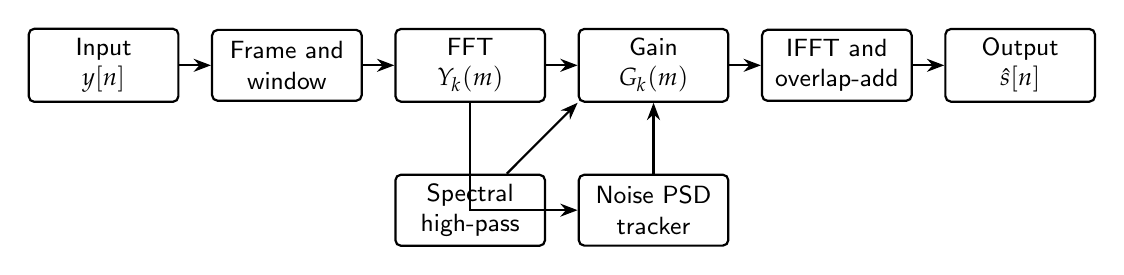
\begin{tikzpicture}[
  box/.style={draw,thick,rounded corners=2pt,minimum height=9mm,minimum width=19mm,align=center,font=\sffamily\small},
  line/.style={-{Stealth[length=2.2mm]},thick}]
\node[box] (in) {Input\\$y[n]$};
\node[box,right=4mm of in] (frame) {Frame and\\window};
\node[box,right=4mm of frame] (fft) {FFT\\$Y_k(m)$};
\node[box,right=4mm of fft] (gain) {Gain\\$G_k(m)$};
\node[box,right=4mm of gain] (ifft) {IFFT and\\overlap-add};
\node[box,right=4mm of ifft] (out) {Output\\$\hat s[n]$};
\node[box,below=9mm of gain] (track) {Noise PSD\\tracker};
\node[box,below=9mm of fft] (hp) {Spectral\\high-pass};
\draw[line] (in) -- (frame);
\draw[line] (frame) -- (fft);
\draw[line] (fft) -- (gain);
\draw[line] (gain) -- (ifft);
\draw[line] (ifft) -- (out);
\draw[line] (fft) |- (track.west);
\draw[line] (track) -- (gain);
\draw[line] (hp) -- (gain.south west);
\end{tikzpicture}
\caption{Signal path. The noise tracker and the high-pass act on the spectrum; the gain is applied to the noisy coefficient and the result is overlap-added.}
\label{fig:blocks}
\end{figure}

\subsection{Framing, windows, and overlap-add}
The input is cut into frames of $N=512$ samples (32~ms) with a hop of $H=256$ samples (16~ms,
50\% overlap). Each frame is multiplied by a square-root Hann window $w[n]$ and transformed with a
radix-2 FFT of length $N$, giving $N/2+1=257$ bins spaced $f_s/N=31.25$~Hz apart:
\begin{equation}
Y_k(m)=\sum_{n=0}^{N-1} w[n]\,y[mH+n]\,e^{-j2\pi kn/N}.
\end{equation}
After the gain is applied, each frame is transformed back, multiplied by the same window, and
added to the output at its position. With a square-root Hann window and 50\% overlap, $w^2$ sums
to one, so an unmodified signal is reconstructed exactly. A frame length of 32~ms is the usual
compromise: short enough that speech is close to stationary within a frame, long enough to
resolve the harmonics of a voice. The ablation in Section~\ref{sec:ablation} confirms it
against 16~ms and 64~ms frames.

\subsection{Pre-filter}
Energy below about 80~Hz is rumble and handling noise and carries no speech information. Two
implementations of an 80~Hz second-order Butterworth high-pass are available.
\begin{itemize}
\item A \emph{causal biquad} in direct form. It adds a frequency-dependent phase shift of tens of
degrees at 100 to 300~Hz. When the result is compared with an unfiltered clean reference, this phase shift
counts as error.
\item A \emph{zero-phase spectral mask} with the same magnitude response, applied as a real per-bin gain. A real,
positive gain has no phase, so the speech is not shifted. The development data selected this
variant, and the ablation confirms it (Section~\ref{sec:ablation}).
\end{itemize}
The magnitude of the 80~Hz second-order Butterworth high-pass, sampled at the bin centres, is
\begin{equation}
|H(f)|=\Bigl[1+\bigl(\tan(\pi f_c/f_s)/\tan(\pi f/f_s)\bigr)^{4}\Bigr]^{-1/2}.
\end{equation}

\subsection{Noise power tracking}
All gain rules need the noise power spectrum $\lambda_d(k,m)$. It cannot be measured directly
while speech is present, so it is tracked from the noisy signal. Two trackers are implemented.

\paragraph{Minimum statistics.} The periodogram $|Y_k(m)|^2$ is smoothed recursively over time,
and the smoothed value is minimised over a sliding window of up to 96 frames (about 1.5~s), kept as six
sub-windows of 16 frames. Because the minimum of a random signal is biased low, the result is multiplied by a
bias factor computed for stationary Gaussian noise. The assumption is that within 1.5~s the
signal falls to the noise floor at least once in every bin.

\paragraph{Minima-controlled recursive averaging (MCRA).} The smoothed periodogram $S(k,m)$ is
divided by its running minimum $S_\mathrm{min}(k,m)$. If the ratio exceeds a threshold $\delta$,
speech is declared present in that cell. The presence indicator is smoothed into a probability $p(k,m)$,
and the noise estimate is updated with a rate that is slow when speech is likely and fast when it is not:
\begin{equation}
\lambda_d(k,m)=\alpha_d(k,m)\,\lambda_d(k,m-1)+\bigl(1-\alpha_d(k,m)\bigr)\,|Y_k(m)|^2,
\end{equation}
with $\alpha_d=\alpha_d^0+(1-\alpha_d^0)\,p(k,m)$. The threshold selected on development data
is $\delta=\valMcraDelta$.

\paragraph{Rise-rate limit.} A minimum tracker jumps upward when the last pause leaves its
window during continuous speech, and the noise estimate then follows the speech. The limit lets the estimate fall at
once but rise by at most \valRiseLimit\dB{} per second. The limit is optional and was selected on
development data; Section~\ref{sec:ablation} shows its effect on the test data.

\begin{figure}[htbp]
\centering
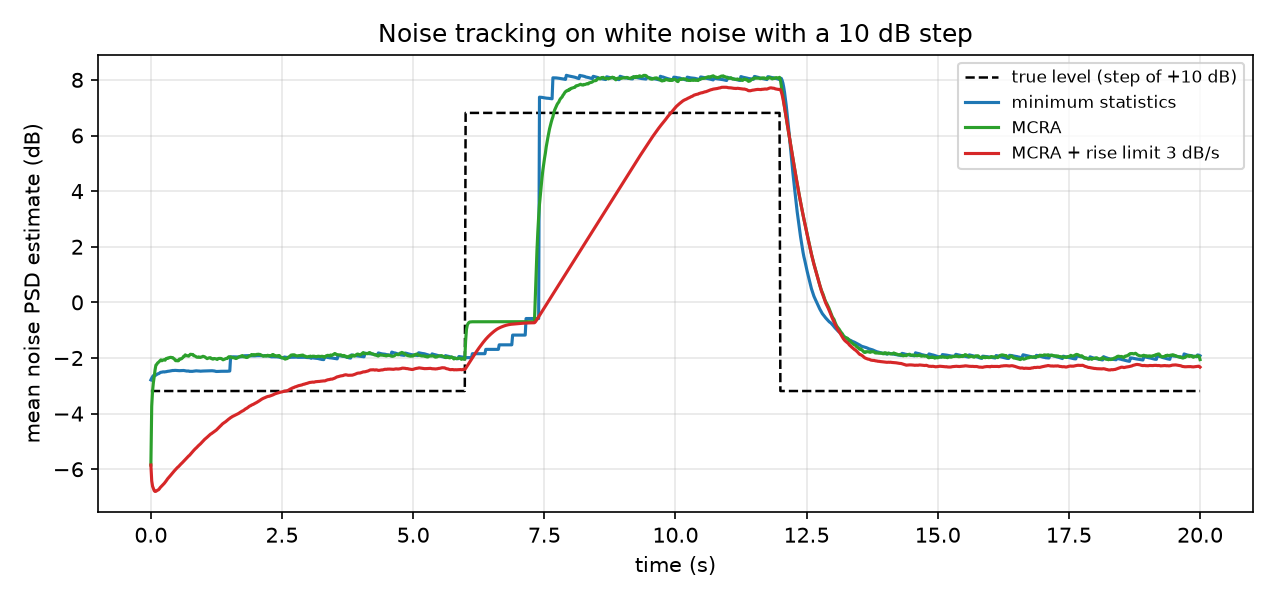
\includegraphics[width=0.82\textwidth]{fig_noise_tracking.png}
\caption{Tracking of white noise with a 10~dB step up and down. The rise limit makes the estimate follow an increase slowly, which protects speech and delays recovery after a genuine noise increase.}
\label{fig:tracking}
\end{figure}

\subsection{Gain rules}
Let $\gamma_k(m)=|Y_k(m)|^2/\lambda_d(k,m)$ be the a posteriori SNR and $\xi_k(m)$ the a priori
SNR. Every rule returns a gain $G$ with $g_\mathrm{min}\le G\le 1$ and the enhanced coefficient is $G\,Y$.

\paragraph{Magnitude spectral subtraction (B1).}
$G=\max\bigl(1-a/\sqrt{\gamma},\;g_\mathrm{min}\bigr)$ with over-subtraction factor $a$. The tuned value is $a=\valOneA$
and the floor is $g_\mathrm{min}=\valOneGMin$.

\paragraph{Wiener gain.}
$G=\xi/(1+\xi)$. The a priori SNR is estimated with the decision-directed approach of Ephraim and Malah:
\begin{equation}
\hat\xi_k(m)=\alpha\,\frac{\hat A_k^2(m-1)}{\lambda_d(k,m-1)}+(1-\alpha)\max\bigl(\gamma_k(m)-1,\,0\bigr),
\end{equation}
where $\hat A_k(m-1)$ is the enhanced amplitude of the previous frame. A value of $\alpha$ close to
one smooths $\xi$ strongly and suppresses isolated bursts of residual noise. The tuned value is
$\alpha=\valDdAlpha$. The recursion starts from zero, so the first frames are attenuated strongly
rather than passed through unattenuated.

\paragraph{Log-spectral amplitude gain.}
$G=\frac{\xi}{1+\xi}\exp\!\bigl(\tfrac12E_1(v)\bigr)$ with $v=\xi\gamma/(1+\xi)$ and $E_1$ the
exponential integral. It is implemented and was part of the structure search on development
data; the search did not select it.

\paragraph{Plain-SNR Wiener gain (B4).} The same Wiener gain with the instantaneous
estimate $\xi=\max(\gamma-1,0)$. It isolates the contribution of decision-directed estimation.

An optional recursive smoother $G\leftarrow\mu G_\mathrm{prev}+(1-\mu)G$ is available. The tuned
value is $\mu=\valGainMu$, that is, none.

\subsection{Streaming implementation}
\label{sec:streaming}
The streaming engine accepts blocks of any length. It keeps the unfinished frame, the
overlap-add tail, the biquad state, and the trackers between calls. Because a sample is final only
after the last frame that contains it has been processed, the output is delayed by $N-1=\valDelaySamples$
samples, that is \valDelayMs~ms at 16~kHz. This delay is constant and independent of the block
size. The streamed output equals the batch output to within \valStreamDiff{} in the largest absolute sample difference,
which is checked by the test suite for the tuned configuration and for random block sizes.

% ------------------------------------------------------------------ 4
\section{Experimental setup}

\subsection{Data}
\paragraph{Speech.} LibriSpeech \emph{dev-clean} is the primary corpus. Development and test
utterances come from disjoint speakers (the split manifest is part of the repository and its
validity is checked in the verification step). The test set has \valNUtt{} utterances with a mean
speech activity of \valActive\% of blocks. The own-voice recording is a secondary corpus: the
first half of the recording provides development segments and the second half provides
\valNOwn{} test segments, with no shared samples.

\paragraph{Noise.} There are \valNNoise{} noise conditions: six synthetic generators (white, pink,
mains hum, babble from four speech sources, amplitude-modulated noise,
and sparse transients), three DEMAND categories (hallway, cafeteria, street traffic), and the
fan and corridor noise recorded by the group. Recordings and DEMAND files are split in time: the first
half serves development, the second half the test.

\paragraph{Cases.} The test set crosses \valNUtt{} utterances, \valNNoise{} noise conditions,
and input SNRs of \valSnrGrid~dB, which gives \valNCases{} cases. Each case has its own seed derived
from its identity, so results do not depend on the number of worker processes. All systems start cold:
there is no noise-only lead-in.

\subsection{Systems}
\begin{description}[leftmargin=1.2cm,labelwidth=1cm]
\item[B0] Unprocessed input.
\item[B1] Spectral subtraction on the same pipeline, with its own tuned parameters.
\item[B2] \file{scipy.signal.wiener}, an external adaptive filter, with a window tuned on development data.
\item[B3] \file{noisereduce} with default settings, an external general-purpose denoiser.
\item[B4] Wiener gain with the plain a priori SNR, on the same pipeline.
\item[B5] HushWave: Wiener gain with decision-directed SNR, MCRA tracking with $\delta=\valMcraDelta$, rise limit \valRiseLimit\dB/s, spectral high-pass, $g_\mathrm{min}=\valGMin$, no gain smoothing, 32~ms frames.
\end{description}
B1 and B4 share every component of B5 except the one that defines them, so differences between
them are attributable to that component. B2 and B3 show how generic tools behave on the same data.

\subsection{Tuning protocol}
Tuning used the \valNTune{} development cases only, with the objective
$J=\tfrac12(\Delta\mathrm{SNR}+\Delta\mathrm{segSNR})$ averaged over cases. The search had three
stages: 24 structures (rule, tracker, pre-filter), a factorial grid over $(g_\mathrm{min},\mu,\alpha)$, and
sweeps of the rise limit, the tracker parameter, and the alternative rule. A first version that varied one parameter at a time missed an interaction
between $g_\mathrm{min}$ and $\mu$; this was found in a rehearsal on development data and the grid was made factorial before the real run.
B1 and B4 were tuned on the same development cases, so that the comparison does not favour B5. Table~\ref{tab:dev} lists the development scores.

\begin{table}[htbp]
\centering
\begin{tabular}{lr}
\toprule
System & DEV objective $J$ (dB) \\
\midrule
B1 spectral subtraction (G1) & 4.65 \\
B2 scipy.signal.wiener & $-$0.29 \\
B3 noisereduce (default) & $-$2.48 \\
B4 Wiener, plain SNR & 4.40 \\
B5 HushWave (full) & 5.06 \\
\bottomrule
\end{tabular}

\caption{Value of the tuning objective on the development set for each system after its own tuning.}
\label{tab:dev}
\end{table}

\subsection{Metrics}
Metrics are computed per case, averaged per utterance, and then across utterances; confidence intervals are 95\% bootstrap intervals over utterances.
The clean reference is cut into blocks of 256 samples. A block is speech-active when its energy is within 40~dB of the loudest block; all others are noise-only.
\begin{itemize}
\item $\Delta$SNR: output SNR minus input SNR against the clean speech (waveform fidelity).
\item $\Delta$segSNR: the same on speech-active blocks, each clamped to $-10$ to 35~dB.
\item NR: energy of the noisy signal over that of the output on noise-only blocks, in dB.
\item SD: distortion of speech blocks, $10\log_{10}(\sum(\hat s-s)^2/\sum s^2)$; lower is better.
\item $\Delta$LSD: change in log-spectral distance on frames that touch speech.
\item MNR: musical-noise ratio, the kurtosis of the noise-only power spectra at the output over that at the input. Values above one mean more isolated spectral peaks than in the input.
\item $\Delta$PESQ (wide-band, ITU-T P.862.2) and $\Delta$STOI from the external packages \file{pesq} (\valPesqVersion) and \file{pystoi} (\valStoiVersion), for B0 to B5 only.
\end{itemize}
These metrics have to be read together: a system that mutes everything scores well on NR and badly on the others.

\subsection{Statistics}
Differences between B5 and a comparison system are tested on per-utterance means with a paired Wilcoxon signed-rank test.
The $p$-values within each family of comparisons are Holm-corrected. The utterance, not the individual case, is the unit of analysis, because
cases built from the same utterance are not independent.

\subsection{Real recordings}
Two recordings (speech in fan noise, speech in corridor noise) have no clean reference, so SNR, PESQ, and STOI cannot be computed.
For these the code measures what the system does to pauses and to speech. A pause block is a block whose energy does not exceed the
95th percentile of the block energies of the matching noise-only recording plus 1~dB; a speech block exceeds that floor by 10~dB.
Reported are the noise reduction and residual level in pauses, the musical-noise ratio in pauses, the change of the speech-block
level, and Welch power spectra of the pauses (computed with the project's own estimator).

% ------------------------------------------------------------------ 5
\section{Results}

\subsection{Overall comparison}
Table~\ref{tab:main} gives the main result and Table~\ref{tab:other} the remaining metrics, both on the test set.

\begin{table}[htbp]
\centering
\small
\setlength{\tabcolsep}{4pt}
\begin{tabular}{lrrr}
\toprule
System & $\Delta$SNR (dB) & $\Delta$segSNR (dB) & $\Delta$PESQ \\
\midrule
B1 spectral subtraction (G1) & 5.20 [4.58, 5.76] & 3.03 [2.42, 3.60] & 0.24 [0.23, 0.26] \\
B2 scipy.signal.wiener & 0.52 [0.32, 0.67] & $-$0.75 [$-$1.04, $-$0.53] & $-$0.04 [$-$0.07, $-$0.02] \\
B3 noisereduce (default) & $-$1.93 [$-$2.22, $-$1.67] & $-$2.46 [$-$2.80, $-$2.15] & $-$0.21 [$-$0.25, $-$0.16] \\
B4 Wiener, plain SNR & 4.74 [4.19, 5.23] & 2.97 [2.35, 3.53] & 0.17 [0.16, 0.18] \\
B5 HushWave (full) & 5.44 [4.81, 6.01] & 3.54 [2.89, 4.14] & 0.25 [0.23, 0.27] \\
\bottomrule
\end{tabular}

\caption{Test set, \valNUtt{} utterances, mean and 95\% interval over utterances.}
\label{tab:main}
\end{table}

\begin{table}[htbp]
\centering
\begin{tabular}{lrrrrr}
\toprule
System & NR (dB) & SD (dB) & $\Delta$LSD (dB) & MNR & $\Delta$STOI \\
\midrule
B1 spectral subtraction (G1) & 9.5 & $-$16.1 & $-$2.89 & 2.16 & 0.006 \\
B2 scipy.signal.wiener & 1.4 & n/a & $-$1.33 & 1.56 & $-$0.011 \\
B3 noisereduce (default) & 21.3 & n/a & 4.89 & 5.04 & $-$0.035 \\
B4 Wiener, plain SNR & 7.2 & $-$19.0 & $-$2.22 & 1.98 & 0.006 \\
B5 HushWave (full) & 10.0 & $-$17.3 & $-$2.85 & 2.56 & 0.003 \\
\bottomrule
\end{tabular}

\caption{Test set, remaining metrics (means). NR: noise reduction, SD: speech distortion, MNR: musical-noise ratio. SD is not defined for B2 and B3.}
\label{tab:other}
\end{table}

HushWave (B5) has the highest SNR improvement, \valDsnrBfive\dB, and the highest segmental SNR improvement, \valSegBfive\dB. Its
advantage over spectral subtraction is small: the median per-utterance difference is \valMedDsnrOne\dB{} in $\Delta$SNR and \valMedSegOne\dB{} in $\Delta$segSNR,
both significant after Holm correction. Against the plain-SNR Wiener gain (B4) the median difference is \valMedDsnrFour\dB,
which measures what decision-directed estimation adds. Table~\ref{tab:tests} lists all paired tests.

\begin{table}[htbp]
\centering
\begin{tabular}{llrrr}
\toprule
Comparison & Metric & Median difference & Holm $p$ & Significant \\
\midrule
B5 vs B1 & $\Delta$SNR & 0.264 & $<$0.001 & yes \\
B5 vs B1 & $\Delta$segSNR & 0.546 & $<$0.001 & yes \\
B5 vs B1 & NR & 0.410 & $<$0.001 & yes \\
B5 vs B1 & $\Delta$PESQ & 0.007 & 0.415 & no \\
B5 vs B1 & $\Delta$STOI & $-$0.002 & $<$0.001 & yes \\
B5 vs B4 & $\Delta$SNR & 0.749 & $<$0.001 & yes \\
B5 vs B4 & $\Delta$segSNR & 0.575 & $<$0.001 & yes \\
B5 vs B4 & NR & 2.650 & $<$0.001 & yes \\
B5 vs B4 & $\Delta$PESQ & 0.080 & $<$0.001 & yes \\
B5 vs B4 & $\Delta$STOI & $-$0.003 & $<$0.001 & yes \\
\bottomrule
\end{tabular}

\caption{Paired Wilcoxon tests of B5 against the two closest systems, on per-utterance means. Positive differences favour B5.}
\label{tab:tests}
\end{table}

\begin{itemize}
\item \textbf{Perceptual quality.} B5 improves PESQ-WB by \valPesqBfive{} (interval \valPesqBfiveCi), which equals spectral subtraction
(\valPesqBone; Holm $p=\valPPesqOne$) and exceeds B4 by \valMedPesqFour. The general-purpose denoiser B3 lowers PESQ by \valPesqBthree.
\item \textbf{Intelligibility.} No gain-based method improves STOI: B1, B4, and B5 change it by about 0.01 or less. B5 is marginally below B1, a
difference that is detectable statistically and negligible in practice. B3 lowers STOI by 0.035.
\item \textbf{Noise reduction against speech preservation.} B3 removes the most noise (\valNrBthree\dB{} against \valNrBfive\dB{} for B5) but at the price of the speech:
its SNR improvement is negative, and on the real recordings it lowers the speech level by \valFanLevelThree\dB{} and \valCorLevelThree\dB.
\end{itemize}

\begin{figure}[htbp]
\centering
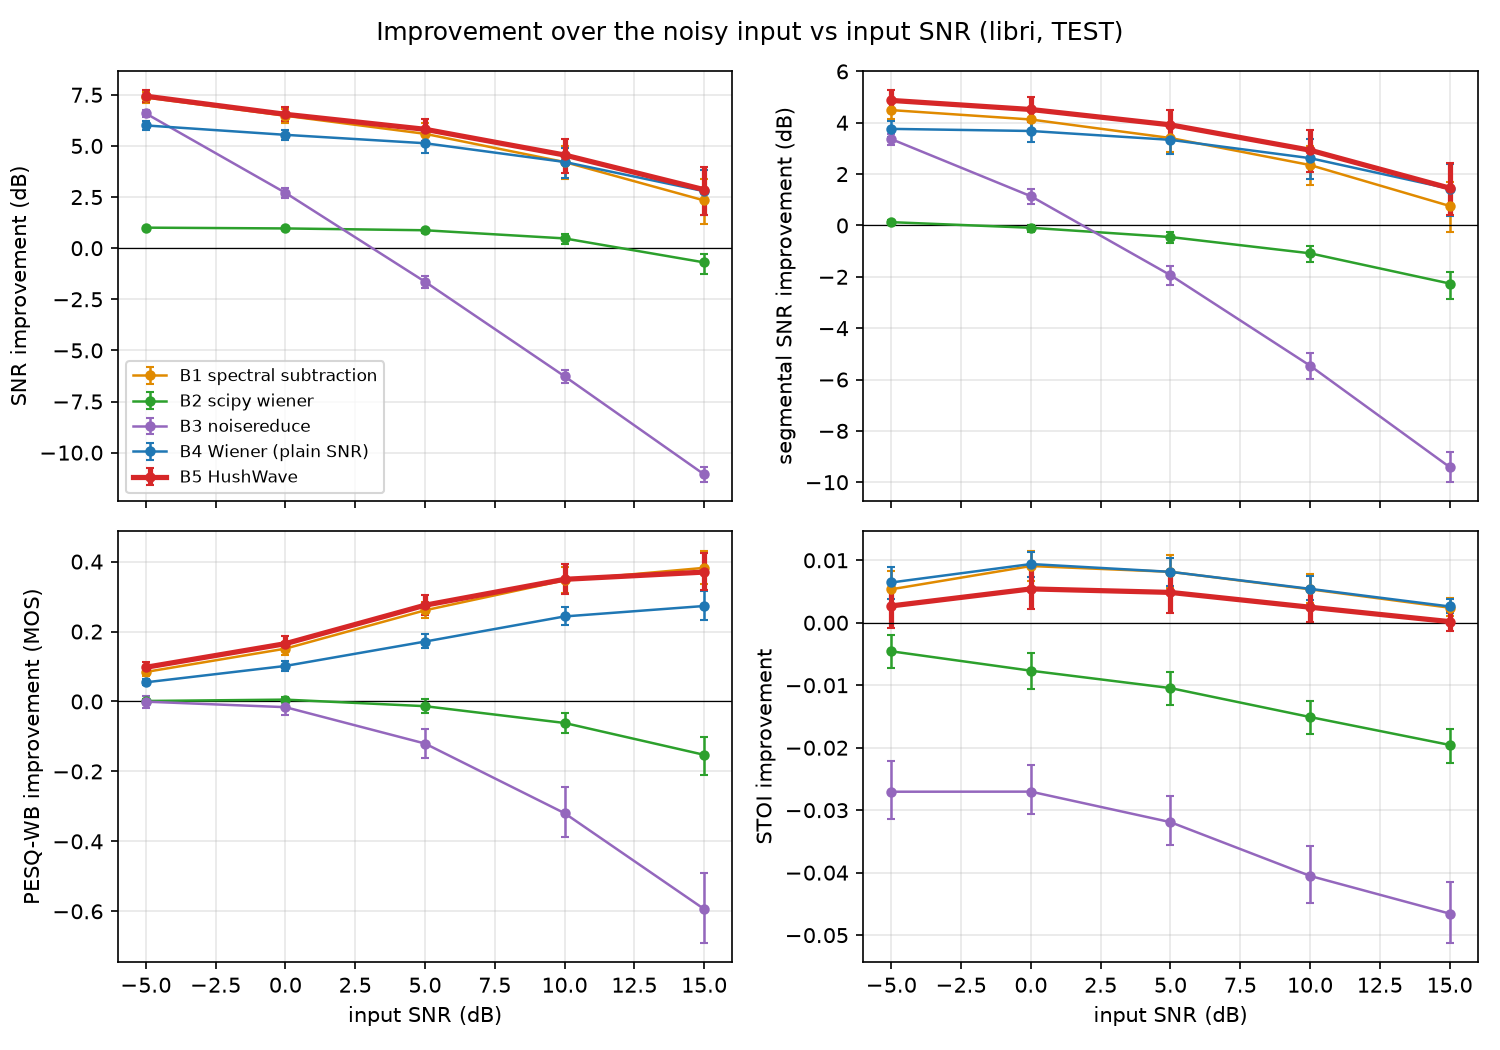
\includegraphics[width=\textwidth]{fig_delta_vs_snr.png}
\caption{Improvement over the noisy input against input SNR, test set, with 95\% intervals over utterances.}
\label{fig:snr}
\end{figure}

\subsection{Dependence on input SNR and noise type}
Figure~\ref{fig:snr} and Table~\ref{tab:snr} show that B5 has the highest mean $\Delta$SNR at every input SNR of the grid, from \valDsnrFiveAtLow\dB{} at \valSnrLow\dB{} down to \valDsnrFiveAtHigh\dB{} at \valSnrHigh\dB.
The improvement shrinks as the input SNR rises because less noise remains to be removed and the risk of distorting speech grows.

\begin{table}[htbp]
\centering
\begin{tabular}{rrrrrr}
\toprule
Input SNR (dB) & B1 & B2 & B3 & B4 & B5 \\
\midrule
$-$5 & 7.37 & 1.00 & 6.59 & 6.00 & 7.43 \\
0 & 6.47 & 0.96 & 2.71 & 5.54 & 6.55 \\
5 & 5.59 & 0.88 & $-$1.64 & 5.13 & 5.81 \\
10 & 4.21 & 0.48 & $-$6.26 & 4.22 & 4.56 \\
15 & 2.33 & $-$0.70 & $-$11.06 & 2.79 & 2.86 \\
\bottomrule
\end{tabular}

\caption{Mean $\Delta$SNR (dB) by input SNR, test set.}
\label{tab:snr}
\end{table}

\begin{figure}[htbp]
\centering
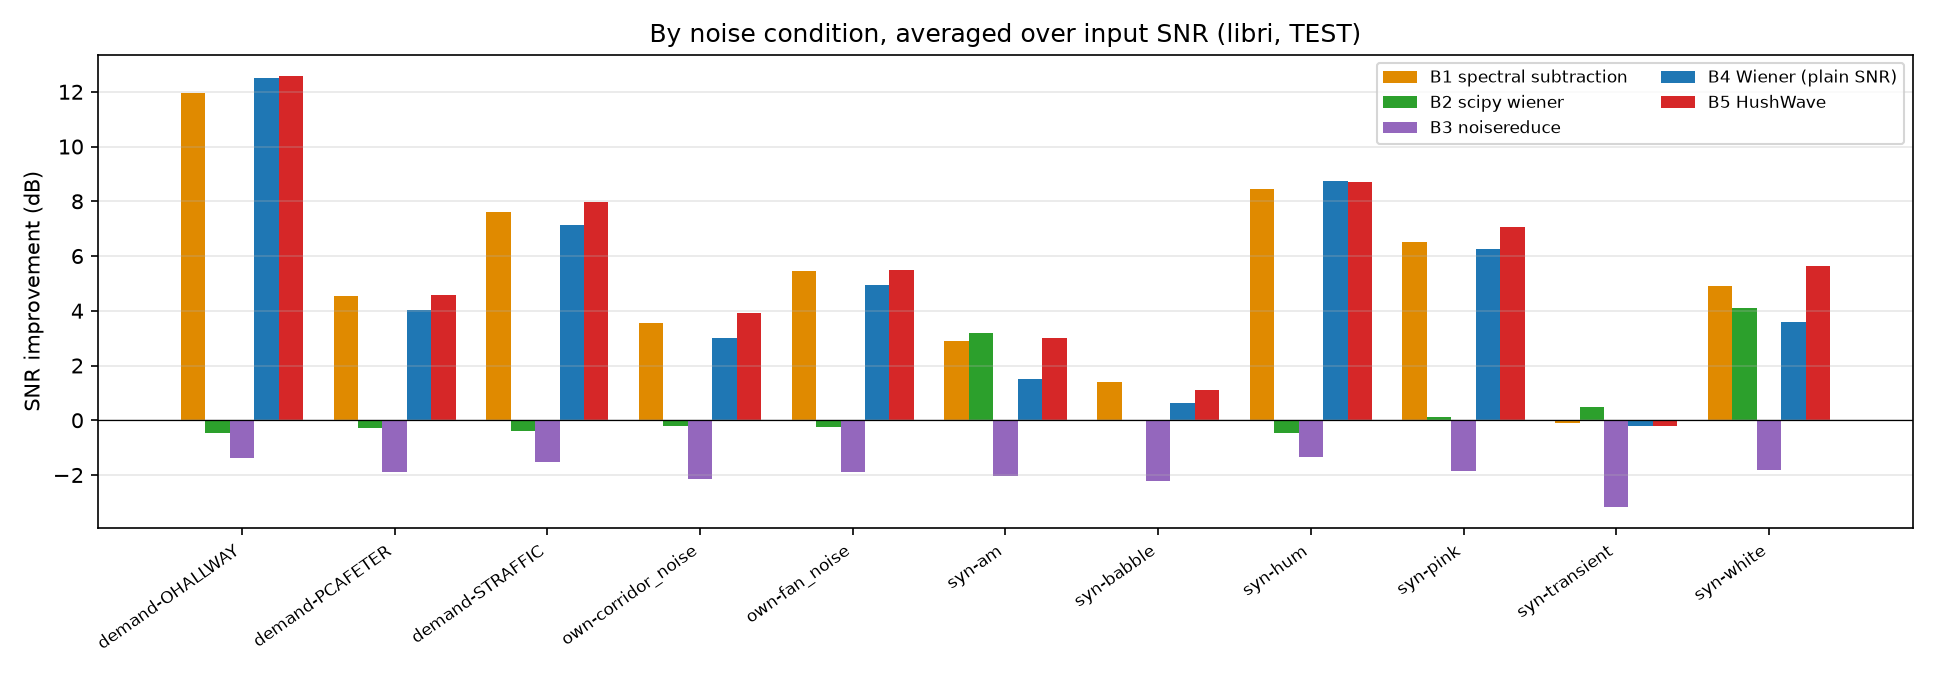
\includegraphics[width=0.95\textwidth]{fig_by_noise.png}
\caption{Mean $\Delta$SNR by noise condition, averaged over input SNR.}
\label{fig:noise}
\end{figure}

By noise type (Table~\ref{tab:noise}, Figure~\ref{fig:noise}), the gain is largest for stationary and narrow-band noises (hum, hallway, white, pink, traffic) and
small for babble and amplitude-modulated noise. Two cases are weak. On the transient noise B5 gives \valTransientFive\dB, that is, no benefit: a minimum-based tracker sees a transient as signal, not as noise. On babble, spectral subtraction is better than B5 (\valBabbleOne\dB{} against \valBabbleFive\dB); babble has the temporal and spectral structure of speech, so any method that separates speech and noise by statistics has little to work with.

\begin{table}[htbp]
\centering
\begin{tabular}{lrrrrr}
\toprule
Noise & B1 & B4 & B5 & B5 NR (dB) & B5 $\Delta$PESQ \\
\midrule
demand-OHALLWAY & 12.0 & 12.5 & 12.6 & 19.9 & 0.29 \\
demand-PCAFETER & 4.6 & 4.0 & 4.6 & 7.9 & 0.14 \\
demand-STRAFFIC & 7.6 & 7.1 & 8.0 & 14.0 & 0.37 \\
own-corridor\_noise & 3.6 & 3.0 & 3.9 & 9.2 & 0.25 \\
own-fan\_noise & 5.4 & 4.9 & 5.5 & 9.0 & 0.22 \\
syn-am & 2.9 & 1.5 & 3.0 & 5.2 & 0.08 \\
syn-babble & 1.4 & 0.6 & 1.1 & 2.7 & 0.01 \\
syn-hum & 8.4 & 8.7 & 8.7 & 18.5 & 0.77 \\
syn-pink & 6.5 & 6.2 & 7.1 & 13.2 & 0.39 \\
syn-transient & $-$0.1 & $-$0.2 & $-$0.2 & 1.3 & $-$0.01 \\
syn-white & 4.9 & 3.6 & 5.6 & 9.2 & 0.25 \\
\bottomrule
\end{tabular}

\caption{Mean $\Delta$SNR (dB) by noise condition, with the noise reduction and $\Delta$PESQ of B5.}
\label{tab:noise}
\end{table}

\subsection{Ablations}
\label{sec:ablation}
Each ablation changes one component of B5 and re-evaluates on the test set with durations held constant (Table~\ref{tab:ablation}, Figure~\ref{fig:ablation}).

\begin{table}[htbp]
\centering
\small
\begin{tabular}{lrrrr}
\toprule
Variant & $\Delta$SNR (dB) & $\Delta$segSNR (dB) & NR (dB) & Holm $p$ \\
\midrule
B5 (full system) & 5.44 [4.81, 6.01] & 3.54 & 10.0 &  \\
gain rule subtraction & 4.62 [3.95, 5.28] & 2.47 & 14.5 & $<$0.001 \\
noise tracker minstats & 5.55 [4.90, 6.15] & 3.56 & 11.7 & 0.011 \\
no rise limit & 5.55 [4.86, 6.22] & 3.22 & 16.6 & 0.604 \\
pre-filter none & 3.77 [3.56, 3.98] & 3.18 & 6.6 & $<$0.001 \\
pre-filter biquad & 1.03 [0.42, 1.60] & $-$0.69 & 9.8 & $<$0.001 \\
weak decision-directed memory & 4.98 [4.40, 5.49] & 3.20 & 7.8 & $<$0.001 \\
lower gain floor & 5.44 [4.81, 6.01] & 3.54 & 10.1 & 1.000 \\
higher gain floor & 5.43 [4.81, 6.00] & 3.50 & 9.7 & 0.003 \\
frame length 16 ms & 5.02 [4.41, 5.60] & 3.19 & 11.5 & $<$0.001 \\
frame length 64 ms & 5.48 [4.85, 6.04] & 3.54 & 9.3 & 1.000 \\
\bottomrule
\end{tabular}

\caption{Test set, B5 and ablations. The last column is the Holm-corrected $p$-value of the paired test against B5 on $\Delta$SNR.}
\label{tab:ablation}
\end{table}

\begin{figure}[htbp]
\centering
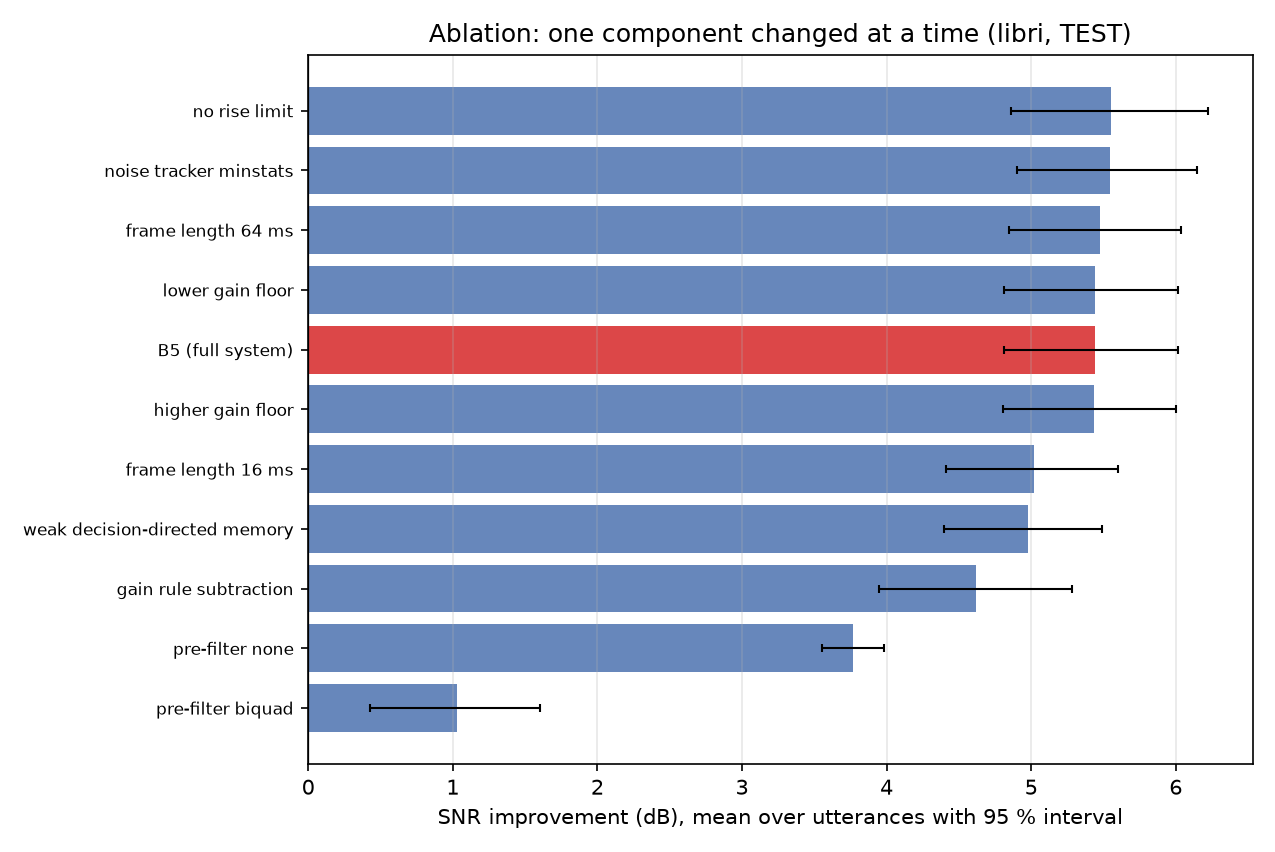
\includegraphics[width=0.9\textwidth]{fig_ablation.png}
\caption{$\Delta$SNR of B5 and its ablations with 95\% intervals.}
\label{fig:ablation}
\end{figure}

\begin{itemize}
\item \textbf{Pre-filter.} Replacing the zero-phase mask by the causal biquad costs \valBiquadLoss\dB{} of SNR improvement, and removing the high-pass costs \valNoneLoss\dB. The two filters have matched magnitudes by design, so the difference is attributed to the phase.
\item \textbf{Rule.} Spectral subtraction with the other components of B5 is worse than the Wiener gain on SNR and on segmental SNR. It removes more noise (Table~\ref{tab:ablation}) but has a higher musical-noise ratio and distorts the speech more.
\item \textbf{Frame length.} 16~ms frames are worse than 32~ms; 64~ms frames are not distinguishable from 32~ms.
\item \textbf{Floor.} Halving $g_\mathrm{min}$ or tripling it changes $\Delta$SNR by 0.01~dB or less.
\item \textbf{Decision-directed smoothing.} Reducing the memory constant from \valDdAlpha{} to 0.5 is worse.
\item \textbf{Tracker.} The minimum-statistics tracker scores about \valMinstatsGain\dB{} \emph{higher} than MCRA in $\Delta$SNR (Holm $p=\valPMinstats$), with similar segmental SNR. MCRA was chosen on development data. On the test data it has more noise reduction, but not a better SNR improvement. This is a selection that the test data does not support on the tuning objective.
\item \textbf{Rise limit.} Without the rise limit the SNR improvement is \valRiseOffDsnr\dB{} against \valDsnrBfive\dB{} with it, which is not a significant difference (Holm $p=\valPRiseOff$). The limit adds about \valRiseOffSeg\dB{} of segmental SNR and \emph{costs} noise reduction: \valNrBfive\dB{} with the limit against \valRiseOffNr\dB{} without it. The limit was chosen by the development objective, which does not see this cost.
\end{itemize}

\subsection{Time-domain and frequency-domain analysis}
\label{sec:timefreq}
Figure~\ref{fig:wave} shows one test case (a cafeteria noise at 5~dB input SNR) in the time domain. The output follows the clean envelope and the noise floor between words is lower, while the strongest speech peaks keep their amplitude.
Figure~\ref{fig:spec} shows the same case as spectrograms: the broad-band noise floor in the input is suppressed in the pauses and between harmonics, and the harmonic structure of the voiced segments is preserved. Residual energy remains in short isolated cells in the pauses, which is what the musical-noise ratio measures, and weak high-frequency speech components are attenuated together with the noise.

\begin{figure}[htbp]
\centering
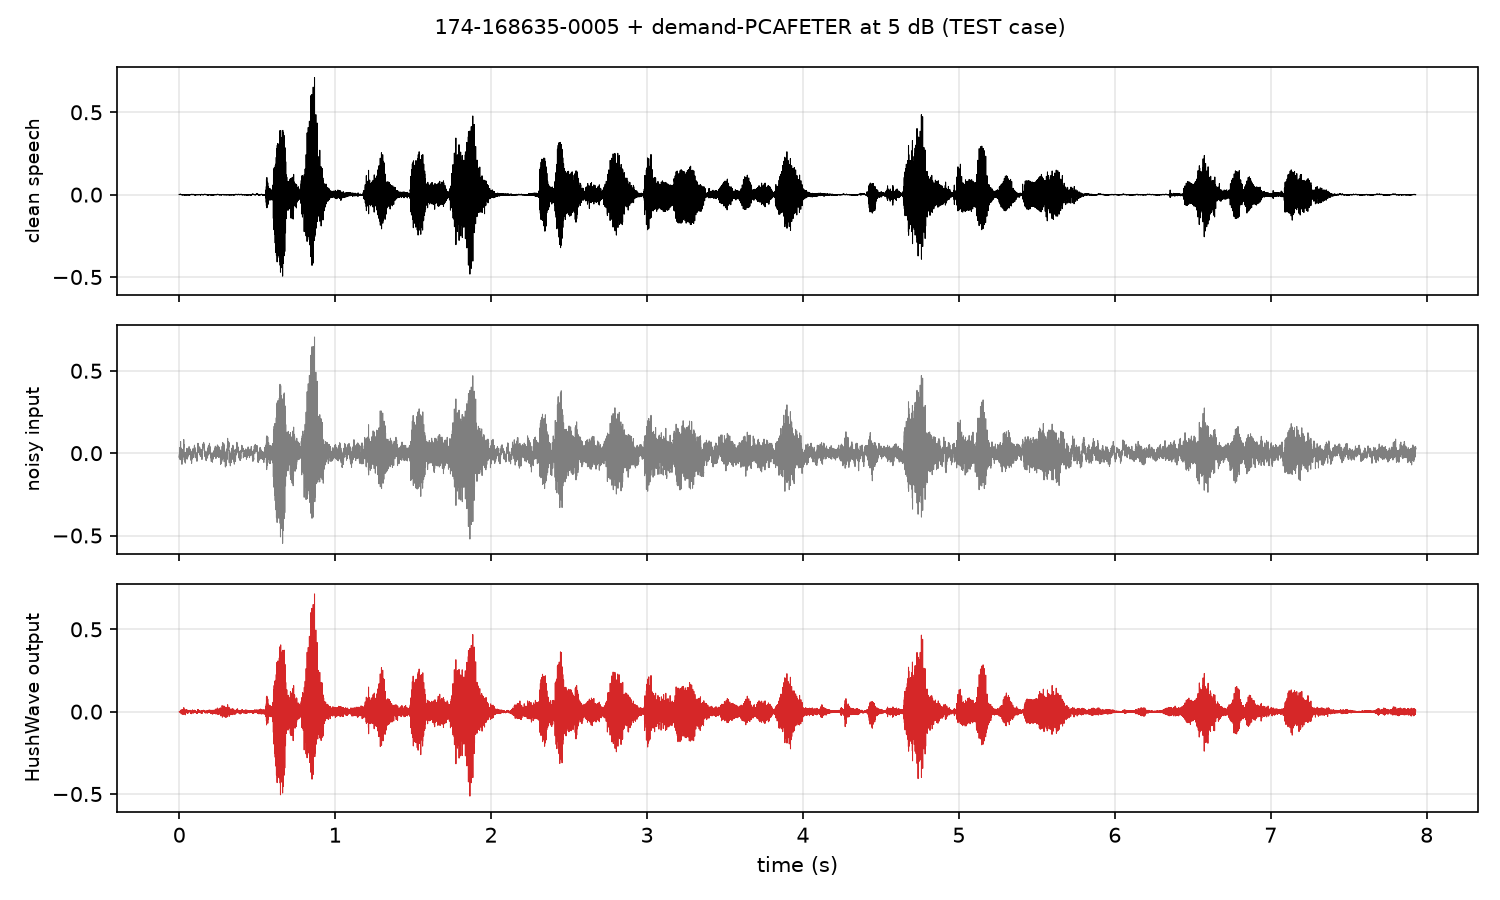
\includegraphics[width=0.92\textwidth]{fig_example_waveforms.png}
\caption{Clean speech, noisy input, and HushWave output for one test case.}
\label{fig:wave}
\end{figure}

\begin{figure}[htbp]
\centering
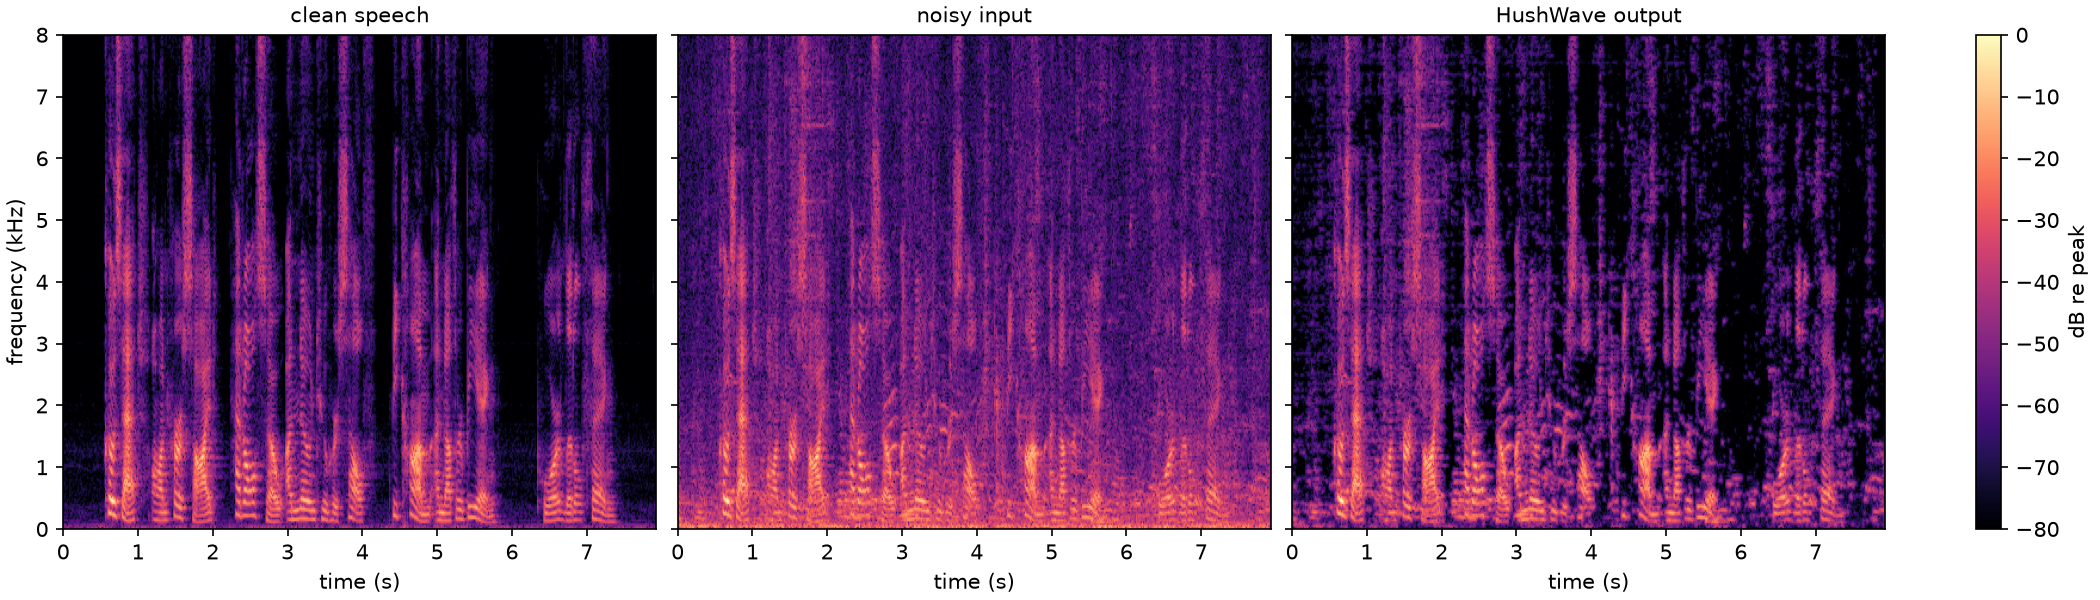
\includegraphics[width=\textwidth]{fig_example_spectrograms.png}
\caption{Spectrograms (dB relative to the peak) of the same case.}
\label{fig:spec}
\end{figure}

Figure~\ref{fig:gain} shows the mean gain per frequency for the same case. The mean gain in speech-active blocks is clearly higher than in noise-only blocks over the whole band, and that difference is what separates speech from noise. Speech-active blocks are still attenuated on average, because many of their cells hold only noise. Both curves fall steeply below 100~Hz, where the high-pass acts.

\begin{figure}[htbp]
\centering
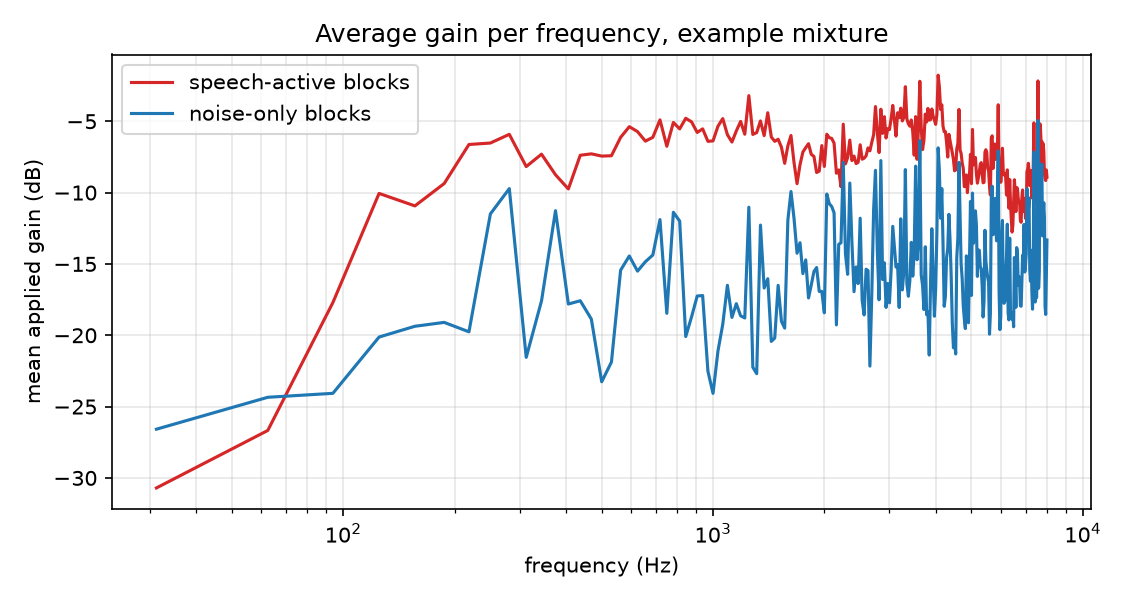
\includegraphics[width=0.7\textwidth]{fig_gain_per_band.png}
\caption{Mean gain applied by B5 per frequency, in speech-active and noise-only blocks.}
\label{fig:gain}
\end{figure}

\subsection{Real recordings}
Table~\ref{tab:real} and Figure~\ref{fig:psd} show the result on the two recordings without a clean reference.

\begin{table}[htbp]
\centering
\small
\begin{tabular}{lrrrr}
\hline
\rowcolor{headfill} \textbf{System} & \textbf{NR in pauses (dB)} & \textbf{Pause level (dBFS)} & \textbf{Speech level (dB)} & \textbf{MNR} \\ \hline
\multicolumn{5}{l}{\emph{Speech in fan noise}} \\ \hline
B1 spectral subtraction & 3.9 & $-$46.1 & $-$0.6 & 2.77 \\ \hline
B2 scipy Wiener & 1.5 & $-$43.6 & $-$0.2 & 2.19 \\ \hline
B3 noisereduce & 15.1 & $-$57.3 & $-$9.8 & 6.85 \\ \hline
B4 Wiener, plain SNR & 2.3 & $-$44.5 & $-$0.1 & 2.11 \\ \hline
B5 HushWave & 2.8 & $-$45.0 & $-$0.2 & 2.87 \\ \hline
\multicolumn{5}{l}{\emph{Speech in corridor noise}} \\ \hline
B1 spectral subtraction & 2.1 & $-$39.7 & $-$0.3 & 1.48 \\ \hline
B2 scipy Wiener & 0.7 & $-$38.3 & $-$0.2 & 0.99 \\ \hline
B3 noisereduce & 20.1 & $-$57.7 & $-$11.3 & 6.39 \\ \hline
B4 Wiener, plain SNR & 1.8 & $-$39.4 & $-$0.1 & 1.33 \\ \hline
B5 HushWave & 1.9 & $-$39.5 & $-$0.2 & 1.42 \\ \hline
\end{tabular}

\caption{Real recordings. NR: noise reduction in pause blocks; pause level relative to full scale; speech level: change of the energy of speech blocks.}
\label{tab:real}
\end{table}

\begin{figure}[htbp]
\centering
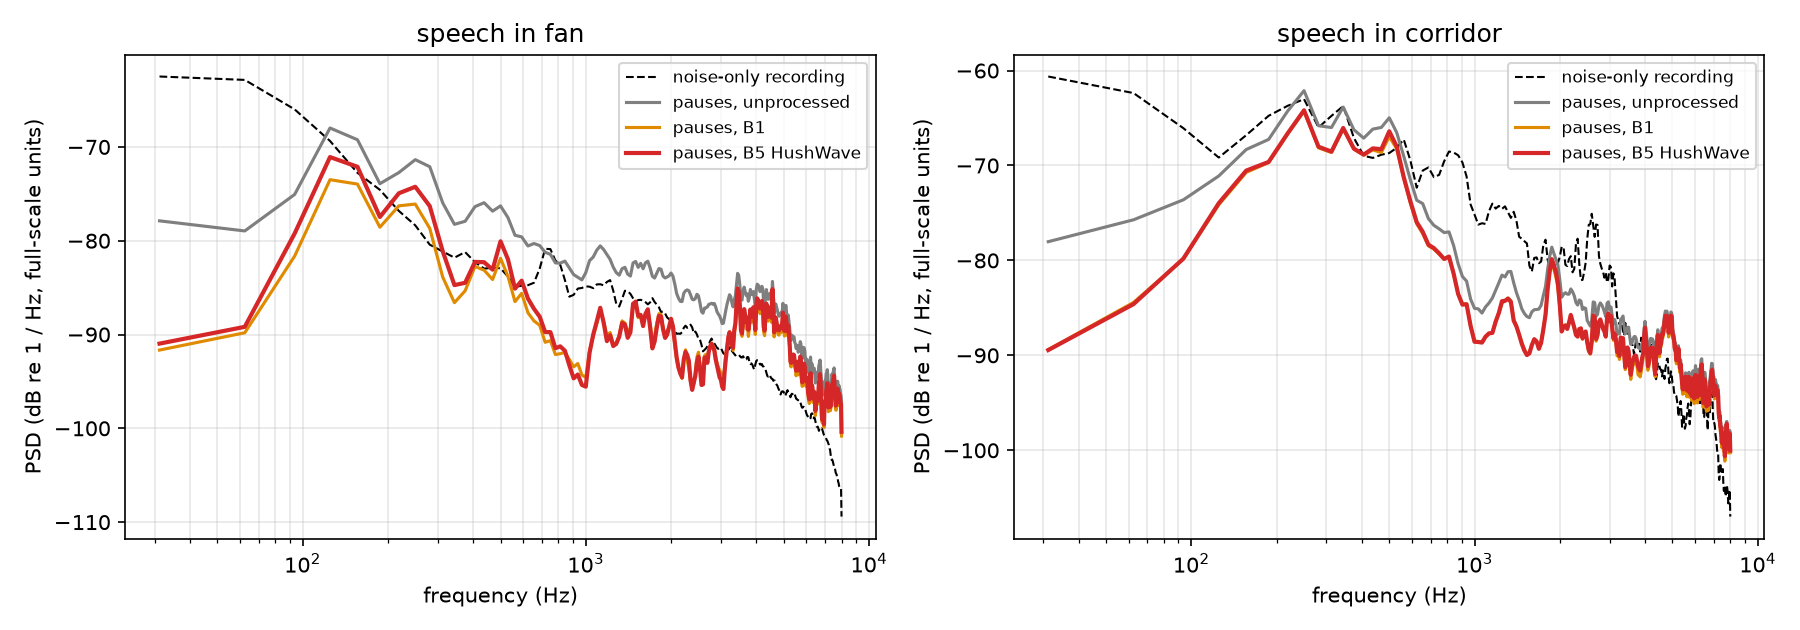
\includegraphics[width=\textwidth]{fig_pause_psd.png}
\caption{Welch power spectra of the pauses before and after processing, with the noise-only recording.}
\label{fig:psd}
\end{figure}

This is the weakest result of the project. HushWave reduces the noise in pauses by only \valFanNrFive\dB{} (fan) and \valCorNrFive\dB{} (corridor), while spectral subtraction reaches
\valFanNrOne\dB{} and \valCorNrOne\dB. For comparison, mixtures of LibriSpeech with the same two noise recordings give a noise reduction of \valFanMixNr\dB{} and \valCorMixNr\dB{} for B5 (Table~\ref{tab:noise}). The two measures are defined differently, but the gap suggests that the continuous speech of these recordings, with few and short pauses, limits the trackers, which then have few moments in which to observe noise alone. We did not isolate this. The spectra in Figure~\ref{fig:psd} show that the reduction is concentrated below 1~kHz, with little change above 3~kHz. We have not tested why; the candidates are low-level speech and breath in the pause blocks and the recording noise floor.
The general-purpose denoiser B3 removes 15 to 20~dB of pause noise, but the speech level falls by about 10 to 11~dB, and its musical-noise ratio is the highest.

\subsection{Own-voice corpus}
On the \valNOwn{} test segments of the own voice (Table~\ref{tab:own}) the ordering is the same as on LibriSpeech: B5 has a mean $\Delta$SNR of \valOwnDsnrFive{} against \valOwnDsnrOne{} for B1. With six segments the intervals are wide and
a Holm-corrected test cannot reach significance, so this corpus supports the direction of the result and nothing more.

\begin{table}[htbp]
\centering
\begin{tabular}{lrr}
\toprule
System & $\Delta$SNR (dB) & $\Delta$segSNR (dB) \\
\midrule
B1 spectral subtraction (G1) & 5.12 [4.04, 5.83] & 3.17 \\
B2 scipy.signal.wiener & 0.64 [0.54, 0.76] & $-$0.57 \\
B3 noisereduce (default) & $-$2.39 [$-$2.56, $-$2.22] & $-$3.29 \\
B4 Wiener, plain SNR & 5.08 [4.33, 5.57] & 3.51 \\
B5 HushWave (full) & 5.53 [4.34, 6.31] & 3.84 \\
\bottomrule
\end{tabular}

\caption{Own-voice test segments, mean and 95\% interval.}
\label{tab:own}
\end{table}

\subsection{Consistency between development and test}
On the development set the tuning objective of B5 is \valJDevFive{} against \valJDevOne{} for B1. On the test set the same quantity is \valJTestFive{} against \valJTestOne. The margin is stable, and there is no sign that the parameters overfit the development data.

\subsection{Latency and real-time performance}
\label{sec:latency}
The algorithmic delay is \valDelayMs~ms (\valDelaySamples{} samples), constant for every block size. Table~\ref{tab:perf} and Figure~\ref{fig:rtf} give the measured cost per block on the machine used for the measurements. For 256-sample (16~ms) blocks the real-time factor is
\valRtf{} and the slowest block takes \valWorstBlock~ms against a budget of \valBlockBudget~ms. The peak memory of a ten-second stream is \valHeapKb~kB. The engine therefore has a large margin on a laptop CPU; these figures describe that one machine and should not be generalised to an embedded target without measurement.

\begin{table}[htbp]
\centering
\begin{tabular}{rrrrr}
\toprule
Block (samples) & Block (ms) & Real-time factor & Worst block (ms) & Budget (ms) \\
\midrule
128 & 8.0 & 0.0218 & 0.43 & 8.0 \\
256 & 16.0 & 0.0204 & 0.56 & 16.0 \\
480 & 30.0 & 0.0193 & 0.76 & 30.0 \\
1024 & 64.0 & 0.0191 & 1.41 & 64.0 \\
\bottomrule
\end{tabular}

\caption{Cost of the streaming engine per block size.}
\label{tab:perf}
\end{table}

\begin{figure}[htbp]
\centering
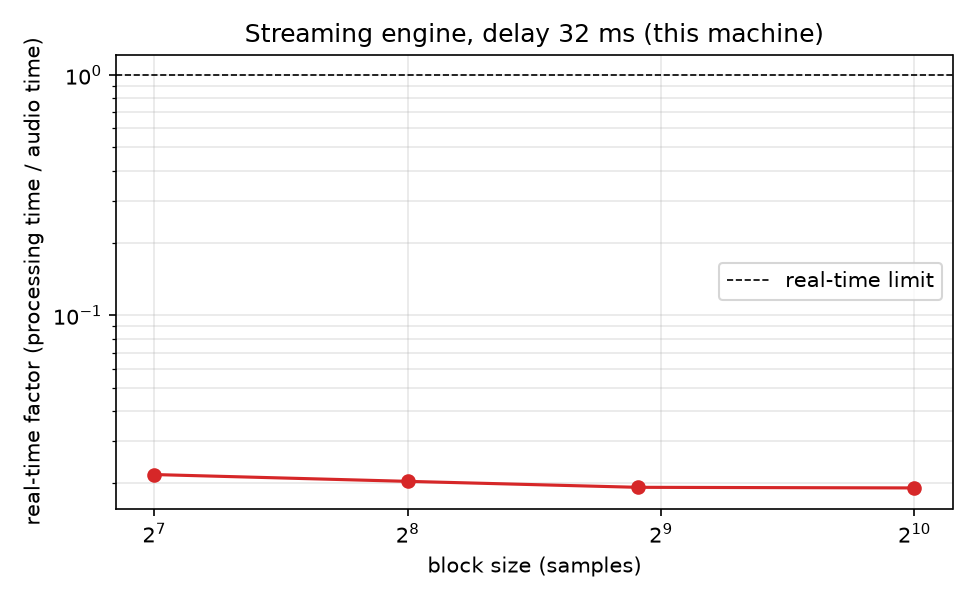
\includegraphics[width=0.62\textwidth]{fig_latency_rtf.png}
\caption{Real-time factor against block size.}
\label{fig:rtf}
\end{figure}

% ------------------------------------------------------------------ 6
\section{Demonstration}
\label{sec:demo}

The demonstration is a local web interface served by the project (\file{make demo-replay} and \file{make demo-live}). The browser acts only as the audio device. In the live mode it captures the microphone at 16~kHz with its own noise suppression,
echo cancellation, and gain control switched off, sends blocks of 256 samples to the Python engine, and plays what returns. All signal processing runs in the same streaming engine that was evaluated, with the frozen tuned settings read from
\file{results/tuning.json}. Nothing is retuned for the demonstration.

\begin{description}[leftmargin=1.2cm,labelwidth=1cm]
\item[Replay.] Two excerpts of the real recordings, each in three versions that share one playback level: the original, spectral subtraction, and HushWave. The versions can be switched during playback without a gap, and a spectrogram of the selected version moves with the playhead.
The excerpts are cut from a continuous run over the whole recording, so they show the system in steady state. The measurements beside them are those of Table~\ref{tab:real}.
\item[Live.] The microphone passes through the engine. An enhancement switch cross-fades between the raw and the enhanced signal, input and output levels are displayed, and the interface reports the algorithmic delay, the processing time per block, the round trip to the engine, the output buffer, and dropouts.
The estimated delay from microphone to headphones adds block, algorithmic delay, round trip, and buffer; it excludes the latency of the audio device. Headphones are required, because speakers feed back into the microphone.
\end{description}
The replay mode needs no microphone and no audio input permission, so the demonstration works even when the live path is unavailable.

% ------------------------------------------------------------------ 7
\section{Discussion and limitations}

\paragraph{What the evidence supports.}
HushWave is the best of the compared systems on waveform measures at every input SNR, and the margin over a well-tuned spectral subtraction is real but small. It matches spectral subtraction on PESQ. It does not improve intelligibility
as measured by STOI, and no method of this family does. The largest benefit of the work is not a new algorithm but a controlled comparison in which each component is isolated and tuned fairly.

\paragraph{Weaknesses.}
\begin{enumerate}
\item The musical-noise ratio of B5 (\valMnrBfive) is the highest of the classical systems (B1 \valMnrBone, B4 \valMnrBfour). The tuning objective cannot see musical noise, and the development data switched gain smoothing off.
\item There is no improvement on transient noise, and spectral subtraction is better on babble.
\item On the real recordings the noise reduction in pauses is no better than that of spectral subtraction (Table~\ref{tab:real}).
\item The rise limit, selected on development data, gives no significant SNR gain on the test data and costs noise reduction. The MCRA tracker, also selected on development data, is slightly worse in $\Delta$SNR than minimum statistics on the test data. Both are listed in the ablation and were not changed after the test evaluation.
\item The own-voice corpus has six segments, which is too few for corrected significance tests.
\end{enumerate}

\paragraph{Threats to validity.}
Test mixtures are synthetic; real conditions add reverberation, non-stationary noise, and microphone characteristics that are absent here. The fan and corridor recordings differ in format (the corridor files are 48~kHz stereo, the others 44.1~kHz dual mono), which digital mixing makes harmless for the mixtures but which deviates from the recording protocol.
The tuning objective is a waveform measure; a perceptual objective could select different parameters. PESQ and STOI come from external packages and were used as published. Timing was measured on one machine.

\paragraph{Possible next steps.} A perceptual or musical-noise term in the tuning objective; a detector that treats transients as noise; longer recordings with more pauses for the real-recording evaluation; and a port of the engine to a fixed-point microcontroller.

% ------------------------------------------------------------------ 8
\section{Conclusion}
A classical single-channel enhancer, implemented from first principles and evaluated under a protocol that prevents tuning on the test data, improves the SNR by \valDsnrBfive\dB{} on average, with a small but statistically consistent advantage over spectral subtraction and without a perceptual gain over it.
The streaming engine meets a real-time budget with a large margin and a delay of \valDelayMs~ms. The results also show the limits of the approach: no intelligibility gain, no help with transient or babble noise, and modest noise reduction on real recordings with few pauses.
These limits are reported as they are.

% ------------------------------------------------------------------ refs
\begin{thebibliography}{99}\small
\bibitem{boll1979} S.~F. Boll, ``Suppression of acoustic noise in speech using spectral subtraction,'' \emph{IEEE Trans. Acoust., Speech, Signal Process.}, vol.~27, no.~2, pp.~113--120, 1979.
\bibitem{ephraim1984} Y.~Ephraim and D.~Malah, ``Speech enhancement using a minimum mean-square error short-time spectral amplitude estimator,'' \emph{IEEE Trans. Acoust., Speech, Signal Process.}, vol.~32, no.~6, pp.~1109--1121, 1984.
\bibitem{ephraim1985} Y.~Ephraim and D.~Malah, ``Speech enhancement using a minimum mean-square error log-spectral amplitude estimator,'' \emph{IEEE Trans. Acoust., Speech, Signal Process.}, vol.~33, no.~2, pp.~443--445, 1985.
\bibitem{martin2001} R.~Martin, ``Noise power spectral density estimation based on optimal smoothing and minimum statistics,'' \emph{IEEE Trans. Speech Audio Process.}, vol.~9, no.~5, pp.~504--512, 2001.
\bibitem{cohen2002} I.~Cohen and B.~Berdugo, ``Noise estimation by minima controlled recursive averaging for robust speech enhancement,'' \emph{IEEE Signal Process. Lett.}, vol.~9, no.~1, pp.~12--15, 2002.
\bibitem{scalart1996} P.~Scalart and J.~V. Filho, ``Speech enhancement based on a priori signal to noise estimation,'' in \emph{Proc. IEEE ICASSP}, 1996, pp.~629--632.
\bibitem{griffinlim1984} D.~W. Griffin and J.~S. Lim, ``Signal estimation from modified short-time Fourier transform,'' \emph{IEEE Trans. Acoust., Speech, Signal Process.}, vol.~32, no.~2, pp.~236--243, 1984.
\bibitem{cooleytukey1965} J.~W. Cooley and J.~W. Tukey, ``An algorithm for the machine calculation of complex Fourier series,'' \emph{Math. Comput.}, vol.~19, no.~90, pp.~297--301, 1965.
\bibitem{welch1967} P.~D. Welch, ``The use of fast Fourier transform for the estimation of power spectra,'' \emph{IEEE Trans. Audio Electroacoust.}, vol.~15, no.~2, pp.~70--73, 1967.
\bibitem{panayotov2015} V.~Panayotov, G.~Chen, D.~Povey, and S.~Khudanpur, ``Librispeech: an ASR corpus based on public domain audio books,'' in \emph{Proc. IEEE ICASSP}, 2015, pp.~5206--5210.
\bibitem{thiemann2013} J.~Thiemann, N.~Ito, and E.~Vincent, ``The diverse environments multi-channel acoustic noise database (DEMAND),'' in \emph{Proc. Meetings on Acoustics}, vol.~19, 2013.
\bibitem{p862} ITU-T Recommendation P.862.2, ``Wideband extension to Recommendation P.862 for the assessment of wideband telephone networks and speech codecs,'' 2007.
\bibitem{taal2011} C.~H. Taal, R.~C. Hendriks, R.~Heusdens, and J.~Jensen, ``An algorithm for intelligibility prediction of time-frequency weighted noisy speech,'' \emph{IEEE Trans. Audio, Speech, Lang. Process.}, vol.~19, no.~7, pp.~2125--2136, 2011.
\bibitem{uemura2009} Y.~Uemura, Y.~Takahashi, H.~Saruwatari, K.~Shikano, and K.~Kondo, ``Automatic optimization scheme of spectral subtraction based on musical noise assessment via higher-order statistics,'' in \emph{Proc. IWAENC}, 2008.
\bibitem{holm1979} S.~Holm, ``A simple sequentially rejective multiple test procedure,'' \emph{Scand. J. Statist.}, vol.~6, no.~2, pp.~65--70, 1979.
\bibitem{wilcoxon1945} F.~Wilcoxon, ``Individual comparisons by ranking methods,'' \emph{Biometrics Bull.}, vol.~1, no.~6, pp.~80--83, 1945.
\end{thebibliography}

% ------------------------------------------------------------------ appendices
\appendix
\section{Reproducing the results}
\label{app:repro}
All commands run from the repository root in a Python 3.11 environment (the results were generated with Python \valPythonVersion, NumPy \valNumpyVersion, SciPy \valScipyVersion, \file{pesq} \valPesqVersion, \file{pystoi} \valStoiVersion, \file{noisereduce} \valNoisereduceVersion).
\begin{center}
\begin{tabular}{@{}ll@{}}
\toprule
Command & Purpose \\
\midrule
\file{make setup} & create the environment \\
\file{make data} & download LibriSpeech and DEMAND, verify checksums \\
\file{make verify} & lint, type check, tests with coverage, results schema, data manifest \\
\file{make experiments} & tune on development data, evaluate once on test data \\
\file{make figures} & draw the figures from the results \\
\file{make results-doc} & write \file{docs/RESULTS.md} \\
\file{make examples} & build the replay clips from the recordings \\
\file{make demo-replay} & start the replay interface \\
\file{make demo-live} & start the live microphone interface \\
\file{make report} & build this report \\
\bottomrule
\end{tabular}
\end{center}

\section{Requirement traceability}
\label{app:trace}
\begin{center}
\small
\begin{tabular}{@{}>{\raggedright\arraybackslash}p{58mm}>{\raggedright\arraybackslash}p{50mm}>{\raggedright\arraybackslash}p{40mm}@{}}
\toprule
Requirement & Where it is met & Code \\
\midrule
One algorithm implemented by the students & Section~\ref{sec:method} & \file{src/hushwave/} \\
Mathematical formulation & Sections~\ref{sec:model} and \ref{sec:method}, \file{docs/THEORY.md} & \file{theory.py} \\
Time-domain analysis & Figure~\ref{fig:wave}, Section~\ref{sec:timefreq} & \file{figures.py} \\
Frequency-domain analysis & Figures~\ref{fig:spec}, \ref{fig:gain}, \ref{fig:psd} & \file{figures.py}, \file{spectral.py} \\
Raw against processed, with numbers & Tables~\ref{tab:main}, \ref{tab:other}, \ref{tab:real} & \file{metrics.py} \\
Justified sampling frequency & Section~\ref{sec:sampling} & \file{theory.py} \\
Working real-time demonstration & Sections~\ref{sec:latency} and \ref{sec:demo} & \file{live.py}, \file{demo\_server.py} \\
\bottomrule
\end{tabular}
\end{center}

\end{document}
